\textbf{\underline{\large{4.4: The Second Derivative: Points of Inflection and Concavity}}} \par

In this section, we are going to take a look at the graphical applications of the second derivative. But first, let's review some definitions: \par

\begin{tcolorbox}[definition]
    \begin{tabbing}
        \textit{Concavity} $\rightarrow$ \= The direction a curve bends. 
    \end{tabbing} \vspace{11pt}
    \begin{tabbing}
        \textit{Concave Up} $\rightarrow$ \= The curve bends counter-clockwise (upwards like a cup) 
    \end{tabbing} \vspace{11pt}
    \begin{tabbing}
        \textit{Concave Down} $\rightarrow$ \= The curve bends clockwise (downwards like a frown)
    \end{tabbing} \vspace{11pt}
    \begin{tabbing}
        \textit{Inflection Value} $\rightarrow$ \= The $x$-value at which the concavity of the curve switches. (Note: \\
        \> this can be a vertical asymptote.)
    \end{tabbing} \vspace{11pt}
    \begin{tabbing}
        \textit{Point of Inflection} $\rightarrow$ \= The point at which the concavity of the curve switches.
    \end{tabbing} 
\end{tcolorbox}

Just as we use the first derivative to find extrema, we use the second derivative to find points of inflection. Therefore, we can say that: \par

\begin{center}
    \fbox{\fbox{\begin{minipage}{0.96 \textwidth}
        \vspace{11pt}
        \begin{center}
            A point of inflection (POI) occurs if and only if the sign of $f''(x)$ changes.
        \end{center}
        \vspace{11pt}
    \end{minipage}}}
\end{center}

\begin{tcolorbox}[objective]
    \begin{center}
        OBJECTIVES \\[11pt]
    \end{center}
    Find Points of Inflection and Intervals of Concavity.
\end{tcolorbox}

Before we attempt any examples, let's take a look at a basic graphical representation of concavity. Take this graph for example: \\

\begin{center}
    
\includegraphics[width = 0.75\textwidth]{\graphicsdir Chapter 4 Graphics/4.4-Graphic1.png}
\end{center}

It appears that this graph is concave down on $(-\infty, \, 4)$ and concave up on $(-4, \, 4) \cup (4, \, \infty)$, more or less. Therefore, $x = -4$ would be an inflection value. Note that $x = 4$ is not an inflection value because the concavity of the graph does not change at that value. \par

\begin{tcolorbox}[example]
    \textbf{Ex 4.4.1: } Find the point(s) of inflection of $y = x^3 + 4x^2 - 3x + 1$.
\end{tcolorbox}
\begin{tcolorbox}[solution]
    \textbf{Sol 4.4.1: } To find the point(s) of inflection of this function, we need to know the sign(s) of the second derivative. We can begin by finding just that. \begin{align*}
        y' &= 3x^2 + 8x - 3 \\[11pt]
        y'' &= 6x + 8
    \end{align*}
    Setting the second derivative equal to zero and making a sign pattern gives us: \begin{align*}
        6x + 8 = 0 \implies x = -\dfrac{4}{3}
    \end{align*} \begin{center}
        \begin{tikzpicture}[baseline=(current bounding box.center)]
            \draw[<->, thick] (0,0) -- (4,0);

            \node at (2,-0.6) {$-\dfrac{4}{3}$};
            \node at (-0.5, -0.6) {$x$};

            \node at (1,0.5) {$-$};
            \node at (2,0.5) {$0$};
            \node at (3,0.5) {$+$};
            \node at (-0.5, 0.5) {$y''$};
        \end{tikzpicture}
    \end{center}
    So, since the sign of the second derivative changes at $x = -\dfrac{4}{3}$, we know that $x = -\dfrac{4}{3}$ is an inflection value. To find the point of inflection, we simply plug this value back into our original equation to obtain our final answer of $\boxed{\left(-\dfrac{4}{3}, \, 5.899\right)}$.
\end{tcolorbox} \vspace{11pt}

\begin{tcolorbox}[example]
    \textbf{Ex 4.4.2: } Find the point(s) of inflection of $y = \dfrac{4x}{x^2 + 1}$.
\end{tcolorbox}
\begin{tcolorbox}[solution]
    \textbf{Sol 4.4.2: } Once again, let's take the second derivative, set it equal to zero, and create a sign pattern. \begin{align*}
        & y' \begin{aligned}[t]
            & = \dfrac{\left(x^2 + 1\right)(4) - (4x)(2x)}{\left(x^2 + 1\right)^2} \\[11pt]
            & = \dfrac{-4x^2 + 4}{\left(x^2 + 1\right)^2}
        \end{aligned} \\[11pt]
        & y'' \begin{aligned}[t]
            & = \dfrac{\left(x^2 + 1\right)^2(-8x) - 2\left(-4x^2 + 4\right)\left(x^2 + 1\right)(2x)}{\left(x^2 + 1\right)^4} \\[11pt]
            & = \dfrac{8x\left(x^2 + 1\right)\left(-\left(x^2 + 1\right) - \left(-2x^2 + 2\right)\right)}{\left(x^2 + 1\right)^4} \\[11pt]
            & = \dfrac{8x\left(x^2 - 3\right)}{\left(x^2 + 1\right)^3}
        \end{aligned}
    \end{align*}
    Setting the second derivative equal to zero and making a sign pattern gives us: \begin{align*}
        \dfrac{8x\left(x^2 - 3\right)}{\left(x^2 + 1\right)^3} = 0 \implies x = 0, \, \pm\sqrt{3}
    \end{align*} \begin{center}
        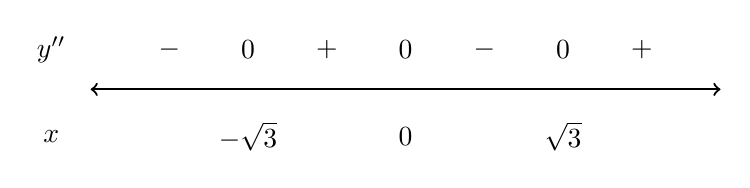
\begin{tikzpicture}[baseline=(current bounding box.center)]
            \draw[<->, thick] (0,0) -- (8,0);

            \node at (2,-0.6) {$-\sqrt{3}$};
            \node at (4,-0.6) {$0$};
            \node at (6,-0.6) {$\sqrt{3}$};
            \node at (-0.5, -0.6) {$x$};

            \node at (1,0.5) {$-$};
            \node at (2,0.5) {$0$};
            \node at (3,0.5) {$+$};
            \node at (4,0.5) {$0$};
            \node at (5,0.5) {$-$};
            \node at (6,0.5) {$0$};
            \node at (7,0.5) {$+$};
            \node at (-0.5, 0.5) {$y''$};
        \end{tikzpicture}
    \end{center}
    Because the sign of the second derivative changes at all of our $x$-values, we know that all of our $x$ values are points of inflections. Plugging these values back into our original equation gives us our final answer of $\boxed{\left(-\sqrt{3}, \, -\sqrt{3}\right), \, (0, \, 0), \, \left(\sqrt{3}, \, \sqrt{3}\right)}$.
\end{tcolorbox} \vspace{11pt}

\begin{tcolorbox}[example]
    \textbf{Ex 4.4.3: } Given the following two sign pattens: \\
    \begin{center}
        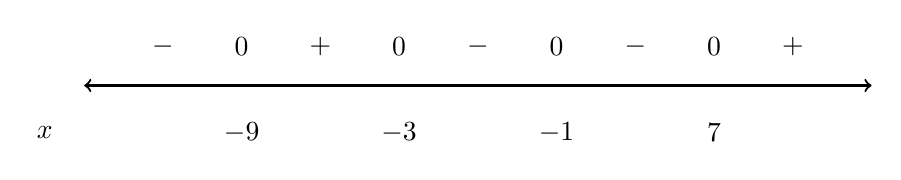
\begin{tikzpicture}[baseline=(current bounding box.center)]
            \draw[<->, thick] (0,0) -- (10,0);

            \node at (2,-0.6) {$-9$};
            \node at (4,-0.6) {$-3$};
            \node at (6,-0.6) {$-1$};
            \node at (8,-0.6) {$7$};
            \node at (-0.5, -0.6) {$x$};

            \node at (1,0.5) {$-$};
            \node at (2,0.5) {$0$};
            \node at (3,0.5) {$+$};
            \node at (4,0.5) {$0$};
            \node at (5,0.5) {$-$};
            \node at (6,0.5) {$0$};
            \node at (7,0.5) {$-$};
            \node at (8,0.5) {$0$};
            \node at (9,0.5) {$+$};
            \node at (-0.5, 0.5) {$\deriv$};
        \end{tikzpicture}
    \end{center} \vspace{11pt} \begin{center}
        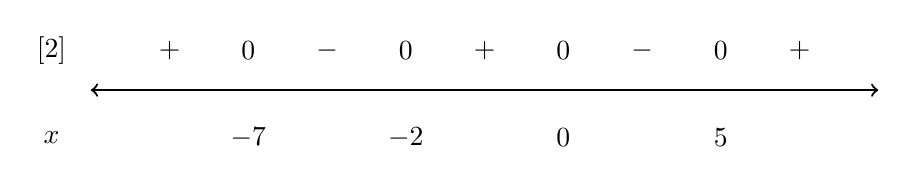
\begin{tikzpicture}[baseline=(current bounding box.center)]
            \draw[<->, thick] (0,0) -- (10,0);

            \node at (2,-0.6) {$-7$};
            \node at (4,-0.6) {$-2$};
            \node at (6,-0.6) {$0$};
            \node at (8,-0.6) {$5$};
            \node at (-0.5, -0.6) {$x$};

            \node at (1,0.5) {$+$};
            \node at (2,0.5) {$0$};
            \node at (3,0.5) {$-$};
            \node at (4,0.5) {$0$};
            \node at (5,0.5) {$+$};
            \node at (6,0.5) {$0$};
            \node at (7,0.5) {$-$};
            \node at (8,0.5) {$0$};
            \node at (9,0.5) {$+$};
            \node at (-0.5, 0.5) {$\deriv[2]$};
        \end{tikzpicture}
    \end{center} \vspace{11pt}
    \begin{enumerate}[label=\hspace{11pt}(\alph*), align=left, leftmargin=*, labelsep=0.25em]
        \item On what interval(s) is $y$ decreasing? \\
        \item On what interval(s) is $y$ concave up? \\
        \item On what interval(s) is $y$ both increasing and concave down?
    \end{enumerate}
\end{tcolorbox}
\begin{tcolorbox}[solution]
    \textbf{Sol 4.4.3:} \par 
    (a) To find the intervals on which $y$ is decreasing, we look for the intervals where the first derivative of $y$ is negative. From our sign pattern, we see that our desired interval is $\boxed{x \in (-\infty, \, -9) \cup (-3, \, 1) \cup (-1, \, 7)}$. \par 
    \vspace{11pt}
    (b) To find the intervals on which $y$ is concave up, we look for the intervals where the second derivative of $y$ is positive. From our sign pattern, we see that our desired interval is $\boxed{x \in (-\infty, \, -7) \cup (-2, \, 0) \cup (5, \, \infty)}$. \par 
    \vspace{11pt}
    (c) To find the intervals on which $y$ is both increasing \textit{and} concave down, we need to take a look at each interval separately and find the intersection (or what's included in both) of the two intervals. From our sign pattern, we know that $y$ is increasing on the interval $x \in (-9, \, -3) \cup (7, \, \infty)$. We also see that $y$ is concave down on the interval $x \in (-7, \, -2) \cup (0, \, 5)$. Taking the intersection of these two intervals gives us our desired answer of $\boxed{x \in (-7, \, -3)}$.
\end{tcolorbox} \vspace{11pt}

\begin{tcolorbox}[example]
    \textbf{Ex 4.4.4: } Find the intervals of concavity for $y = xe^{2x}$. 
\end{tcolorbox}
\begin{tcolorbox}[solution]
    \textbf{Sol 4.4.4: } We begin this problem just like with the others: \begin{align*}
        y' &= x(2)\left(e^{2x}\right) + e^{2x}(1) \\[6pt]
        &= e^{2x}(2x + 1) \\[12pt]
        y'' &= e^{2x}(2) + (2x + 1)(2)\left(e^{2x}\right) \\[6pt]
        &= e^{2x}(2 + (2x + 1)(2)) \\[6pt]
        &= e^{2x}(4x + 4)
    \end{align*}
    Now, let's set the second derivative equal to zero and create a sign pattern: \begin{align*}
        e^{2x}(4x + 4) = 0 \implies x = -1
    \end{align*} \begin{center}
        \begin{tikzpicture}[baseline=(current bounding box.center)]
            \draw[<->, thick] (0,0) -- (4,0);

            \node at (2,-0.6) {$-1$};
            \node at (-0.5, -0.6) {$x$};

            \node at (1,0.5) {$-$};
            \node at (2,0.5) {$0$};
            \node at (3,0.5) {$+$};
            \node at (-0.5, 0.5) {$y''$};
        \end{tikzpicture}
    \end{center}
    From this sign pattern, we conclude that $y$ is \fbox{concave down on $x \in (-\infty, \, -1)$} and \fbox{concave up on $x \in (-1, \, \infty)$}.
\end{tcolorbox} \vspace{11pt}

\begin{tcolorbox}[example]
    \textbf{Ex 4.4.5: } At what point on the curve below is $\deriv < 0$ and $\deriv[2] > 0$? \\
    
    \begin{center}
        
\includegraphics[width=0.85\textwidth]{\graphicsdir Chapter 4 Graphics/4.4-Graphic2.png}
    \end{center}
    \vspace{11pt}
    \begin{oneparchoices}
        \choice $M$ 
        \choice $N$ 
        \choice $O$ 
        \choice $P$ 
        \choice $Q$
    \end{oneparchoices}
\end{tcolorbox}
\begin{tcolorbox}[solution]
    \textbf{Sol 4.4.5: } This problem is very similar to \textbf{Ex 4.4.3}, but instead of sign patterns, we are given a graph. Now, let's break down the information we are given: \par 
    \vspace{11pt}
    First, $\deriv < 0$ implies that the graph is decreasing at our desired point. Already, that information allows us to rule out points $N, O$, and $P$. The second piece of information that we are given is $\deriv[2] > 0$. This means that the curve is concave up at our desired point. From our remaining two points, we see that point $\boxed{Q}$ satisfies this statement indeed.
\end{tcolorbox}

\newpage

\textbf{\large{4.4 Free Response Homework}} \par

\onequestion{1. Given this sign pattern for the second derivative of $F(x)$, on what intervals is $F(x)$ concave down?} \begin{center}
    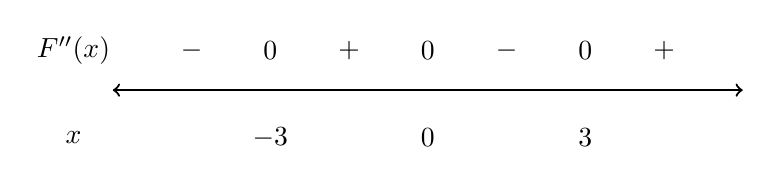
\begin{tikzpicture}[baseline=(current bounding box.center)]
        \draw[<->, thick] (0,0) -- (8,0);

        \node at (2,-0.6) {$-3$};
        \node at (4,-0.6) {$0$};
        \node at (6,-0.6) {$3$};
        \node at (-0.5, -0.6) {$x$};

        \node at (1,0.5) {$-$};
        \node at (2,0.5) {$0$};
        \node at (3,0.5) {$+$};
        \node at (4,0.5) {$0$};
        \node at (5,0.5) {$-$};
        \node at (6,0.5) {$0$};
        \node at (7,0.5) {$+$};
        \node at (-0.5, 0.5) {$F''(x)$};
    \end{tikzpicture}
\end{center} \vspace{11pt}
\onequestion{2. The sign pattern for the derivative of $H(x)$ is given.} \begin{center}
    \begin{tikzpicture}[baseline=(current bounding box.center)]
        \draw[<->, thick] (0,0) -- (8,0);

        \node at (2,-0.6) {$-4$};
        \node at (4,-0.6) {$-1$};
        \node at (6,-0.6) {$2$};
        \node at (-0.5, -0.6) {$x$};

        \node at (1,0.5) {$+$};
        \node at (2,0.5) {$0$};
        \node at (3,0.5) {$-$};
        \node at (4,0.5) {$0$};
        \node at (5,0.5) {$-$};
        \node at (6,0.5) {$0$};
        \node at (7,0.5) {$+$};
        \node at (-0.5, 0.5) {$\dfrac{\dd ^2H}{\dd x^2}$};
    \end{tikzpicture}
\end{center}
\twoquestion{(a) Is $x = -4$ point of inflection?}{(b) Is $x = -1$ a point of inflection?} \\[11pt]

Find point(s) of inflection and interval(s) of concavity for the following equations. \par 

\twoquestion{3. $y = x^3 + x^2 - 7x - 15$}{4. $y = 3x^4 - 20x^3 + 42x^2 - 26x + 16$} \\[11pt]
\twoquestion{5. $y = -\dfrac{4x}{x^2 + 4}$}{6. $y = \dfrac{x^2 - 1}{x^2 - 4}$} \\[11pt]
\twoquestion{7. $y = \ln \left(4x - x^3\right)$}{8. $y = x\sqrt{8 - x^2}$} \\[11pt]
\twoquestion{9. $y = \dfrac{1}{2}x + \sin (x) \bargap x \in (0, \, 2\pi)$}{10. $y = xe^{-x}$} \\[11pt]
\twoquestion{11. $y = e^{-x^2}$}{12. $y = \dfrac{x}{x^2 - 9}$} \\[11pt]
\onequestion{13. $y = 2x - x^{\frac{2}{3}}$} 

\newpage

\textbf{\large{4.4 Multiple Choice Homework}} \par

\begin{questions}
    \question $f(x) = x^3 - 6x^2$ is concave up when: \\

    \begin{oneparchoices}
        \choice $x > 2$
        \choice $x < 2$
        \choice $0 < x < 4$
        \choice $x < 0$ or $x > 4$
        \choice $x > 6$
    \end{oneparchoices} \par \horizontalline

    \question Given the twice differentiable function $f$, which of the following statements is true? \begin{center}
        \begin{tikzpicture}
        % Created with Gemini

        % Axes
        \draw[thick, ->] (-0.5, 0) -- (4, 0) node[below right] {$x$};
        \draw[thick, ->] (0, -2) -- (0, 3) node[left] {$y$};

        % The Curve f(x)
        % Using a plot of an exponential-like decay for that specific curvature
        \draw[ultra thick, name path=curve] (0, 2) .. controls (0.5, 0.5) and (1.5, -1) .. (4, -1.2);

        % Label for f(x)
        \node at (1.8, 1.8) {\large $f(x)$};

        % Find intersection with x-axis to place 'a'
        \path[name path=xaxis] (-0.5, 0) -- (4, 0);
        \fill [name intersections={of=curve and xaxis, by=intersect}]
            (intersect) circle (1pt);

        % Draw the tick mark and label 'a'
        \draw[thick] ([yshift=5pt]intersect) -- ([yshift=-5pt]intersect) 
            node[below right, yshift=-2pt] {\large $a$};

        \end{tikzpicture}
    \end{center} \vspace{11pt}

    \begin{oneparchoices}
        \choice $f'(a) < f''(a) < f(a)$
        \choice $f'(a) < f(a) < f''(a)$
        \choice $f''(a) < f(a) < f'(a)$ \\[11pt]
        \makebox[0.19\textwidth] \choice $f''(a) < f'(a) < f(a)$
        \makebox[0.17\textwidth] \choice $f(a) < f'(a) < f''(a)$
    \end{oneparchoices} \par \horizontalline

    \question For $x > 0$, let $f'(x) = \dfrac{\ln x}{x}$ and $f''(x) = \dfrac{1 - \ln x}{x^2}$. Which of the following is true? \\

    \begin{oneparchoices}
        \choice $f$ is decreasing for $x > 1$ and the graph of $f$ is concave down for $x > e$. \\[11pt]
        \makebox[0.035\textwidth] \choice $f$ is decreasing for $x > 1$ and the graph of $f$ is concave up for $x > e$. \\[11pt]
        \makebox[0.035\textwidth] \choice $f$ is increasing for $x > 1$ and the graph of $f$ is concave down for $x > e$. \\[11pt]
        \makebox[0.035\textwidth] \choice $f$ is increasing for $x > 1$ and the graph of $f$ is concave up for $x > e$. \\[11pt]
        \makebox[0.035\textwidth] \choice $f$ is increasing for $0 < x < e$ and is concave down for $0 < x < e^{\frac{3}{2}}$.
    \end{oneparchoices} \par \horizontalline

    \question Consider the function $f(x) = \left(x^2 - 5\right)^3$ for all real numbers $x$. The number of inflection points for the graph of $f$ is \\ 

    \begin{oneparchoices}
        \choice $1$
        \choice $2$
        \choice $3$
        \choice $4$
        \choice $5$
    \end{oneparchoices} \par \horizontalline

    \question If $\diff [f(x)] = g(x)$ and $\diff [g(x)] = f(3x)$, then $\dfrac{\dd ^2}{\dd x^2} \left[f\left(x^2\right)\right]$ is \\

    \begin{oneparchoices}
        \choice $4x^2f\left(3x^2\right) + 2g\left(x^2\right)$
        \choice $f\left(3x^2\right)$
        \choice $f\left(x^4\right)$ \\[11pt]
        \makebox[0.19\textwidth] \choice $2xf\left(3x^2\right) + 2g\left(x^2\right)$
        \makebox[0.24\textwidth] \choice $2xf\left(3x^2\right)$
    \end{oneparchoices} \par \horizontalline

    \question If $y = e^{kx}$, then $\deriv[5] = $ \\

    \begin{oneparchoices}
        \choice $k^5e^k$
        \choice $k^5e^{kx}$
        \choice $5!e^{kx}$
        \choice $5!e^{x}$
        \choice $5e^{kx}$
    \end{oneparchoices} \par \horizontalline

    \question The graph of $y = 3x^5 - 10x^4$ has an inflection point at \\

    \begin{oneparchoices}
        \choice $(0, \, 0)$ only
        \choice $(3, \, -81)$ only
        \choice $(2, \, -6)$ only \\[11pt]
        \makebox[0.18\textwidth] \choice $(0, \, 0)$ and $(2, \, -64)$
        \makebox[0.21\textwidth] \choice $(0, \, 0)$ and $(3, \, -81)$
    \end{oneparchoices} \par \horizontalline

    \question An equation of the line tangent to the graph of $y = x^3 + 3x^2 + 2$ at its point of inflection is \\

    \begin{oneparchoices}
        \choice $y = -3x + 1$
        \choice $y = -3x = 7$
        \choice $y = x + 5$ \\[11pt]
        \makebox[0.25\textwidth] \choice $y = 3x + 1$
        \makebox[0.28\textwidth] \choice $y = 3x + 7$
    \end{oneparchoices} \par \horizontalline

    \question The number of inflection points for the graph of $y = 2x + \cos \left(x^2\right)$ in the interval $0 \leq x \leq 5$ is \\

    \begin{oneparchoices}
        \choice $6$
        \choice $7$
        \choice $8$
        \choice $9$
        \choice $10$
    \end{oneparchoices} \par \horizontalline

    \question On which of the following intervals is the graph of the curve $y = x^5 - 5x^4 + 10x + 15$ concave up? \begin{center}
        $\hfill \text{I. $x < 0$} \hfill \text{II. $0 < x < 3$} \hfill \text{III. $x > 3$} \hfill$
    \end{center} \vspace{11pt}

    \begin{oneparchoices}
        \choice I only
        \choice II only
        \choice III only
        \choice I and II only
        \choice II and III only
    \end{oneparchoices} \par \horizontalline

    \question Let $f$ be a function with a second derivative given by $f''(x) = x^2(x - 3)(x - 6)$. What are the $x$-coordinates of the points of inflection of the graph of $f$? \\

    \begin{oneparchoices}
        \choice $0$ only
        \choice $3$ only
        \choice $0$ and $6$ only
        \choice $3$ and $6$ only
        \choice $0$, $3$, and $6$
    \end{oneparchoices} \par \horizontalline

    \question The derivative of a function is given by $f'(x) = x^2\cos \left(x^2\right)$. How many points of inflection does the graph of $f$ have on the open interval $(-2, \, 2)$? \\

    \begin{oneparchoices}
        \choice $1$
        \choice $2$
        \choice $3$
        \choice $4$
        \choice $5$
    \end{oneparchoices} \par \horizontalline

    \question How many points of inflection does the graph of $y = \cos (x) + \dfrac{1}{3}\cos (x) - \dfrac{1}{5}\cos (5x)$ have on the interval $0 \leq x \leq \pi$? \\

    \begin{oneparchoices}
        \choice $1$
        \choice $2$
        \choice $3$
        \choice $4$
        \choice $5$
    \end{oneparchoices} \par \horizontalline

    \question At what point on the curve below is $\deriv > 0$ and $\deriv[2] > 0$? 
    \begin{center}
        
\includegraphics[width = 0.6\textwidth]{\graphicsdir Chapter 4 Graphics/4.4-Graphic2.png}
    \end{center} \vspace{11pt}

    \begin{oneparchoices}
        \choice $M$
        \choice $N$
        \choice $O$
        \choice $P$
        \choice $Q$
    \end{oneparchoices} \par \horizontalline

    \question At what point on the curve below is $\deriv < 0$ and $\deriv[2] < 0$? 
    \begin{center}
        
\includegraphics[width = 0.6\textwidth]{\graphicsdir Chapter 4 Graphics/4.4-Graphic2.png}
    \end{center} \vspace{11pt}

    \begin{oneparchoices}
        \choice $M$
        \choice $N$
        \choice $O$
        \choice $P$
        \choice $Q$
    \end{oneparchoices} \par \horizontalline

    \question The graph of the function f(x) is shown below. At which point on the graph of $f(x)$ is $f'(x) > 0$ and $f''(x) < 0$?
    \begin{center}
        
\includegraphics[width = 0.6\textwidth]{\graphicsdir Chapter 4 Graphics/4.4-Graphic3.png}
    \end{center} \vspace{11pt}

    \begin{oneparchoices}
        \choice $A$
        \choice $B$
        \choice $C$
        \choice $D$
        \choice $E$
    \end{oneparchoices} \par \horizontalline

    \question At which of the five points on the graph in the figure below is $\deriv$ and $\deriv[2]$ both negative? 
    \begin{center}
        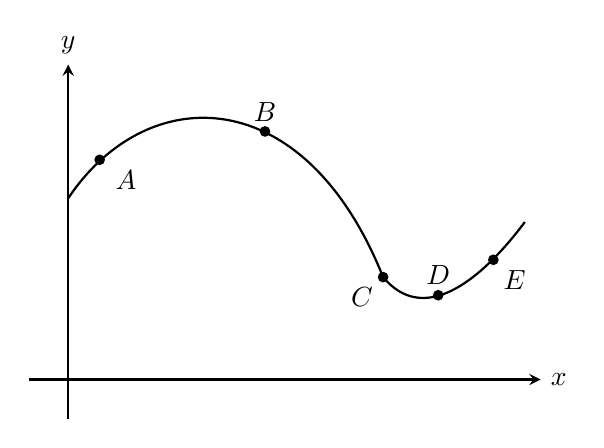
\begin{tikzpicture}[>=stealth, thick]
            % Generated with Gemini

            % Axes
            \draw[->] (-0.5, 0) -- (6, 0) node[right] {$x$};
            \draw[->] (0, -0.5) -- (0, 4) node[above] {$y$};

            % The Curve
            \draw[thick] (0, 2.3) .. controls (1, 3.8) and (3, 3.8) .. (4, 1.3) 
                                .. controls (4.5, 0.7) and (5.2, 1.2) .. (5.8, 2);

            % Point A - Above the curve
            \filldraw (0.4, 2.79) circle (1.5pt) node[below right, xshift=2pt] {$A$};
            
            % Point B - Slightly below the curve
            \filldraw (2.5, 3.15) circle (1.5pt) node[above] {$B$};
            
            % Point C - On the curve
            \filldraw (4.0, 1.3) circle (1.5pt) node[below left] {$C$};
            
            % Point D - Floating above the valley
            \filldraw (4.7, 1.07) circle (1.5pt) node[above] {$D$};
            
            % Point E - On the curve (rising edge)
            \filldraw (5.4, 1.52) circle (1.5pt) node[below right] {$E$};

        \end{tikzpicture}
    \end{center} \vspace{11pt}

    \begin{oneparchoices}
        \choice $A$
        \choice $B$
        \choice $C$
        \choice $D$
        \choice $E$
    \end{oneparchoices} \par \horizontalline
\end{questions}